\section{Experiments}
\label{sec:experiments}

\noindent\textbf{Protocol.} Clean accuracy is measured on the 3,000 held-out images, and dev accuracy on 900 images (\cref{sec:v4}). Test accuracy comes from the leaderboard and exists only for submitted models. For the others we report how many test images are predicted real (500 of 1,500 expected). Every model runs once on the unmodified $512^2$ image.

\begin{table}[t]
  \centering\small
  \setlength{\tabcolsep}{2.6pt}
  \begin{tabular}{@{}lccccc@{}}
    \toprule
    Model & Crop & Clean & Dev & Test & \#real \\
    \midrule
    Baseline (no aug.)          & 512 & \textbf{100} & \textbf{100} & 33.3$^\dagger$ & 1500 \\
    Ours + $128^2$ crops        & 128 & 99.9 & 96.0 & -- & 551 \\
    \textbf{Ours (submitted)}   & 256 & 99.7 & 96.1 & \textbf{95.3} & 536 \\
    \bottomrule
  \end{tabular}
  \caption{\textbf{Main results} (accuracy, \%). \emph{\#real}: test images predicted real (500 expected). $^\dagger$All 1,500 test images predicted real, which scores $1/3$ on the balanced test set.}
  \label{tab:main}
\end{table}

\subsection{Main result}
The baseline is perfect on clean and dev data but labels every test image as real (\cref{tab:main}). Our model gives up 0.3 points of clean accuracy and scores 96.1\% on dev and \textbf{96.33\%} (1,429/1,500) on test. Dev predicted the test score closely.

\begin{figure}[t]
  \centering
  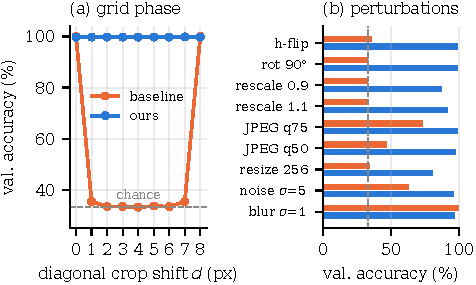
\includegraphics[width=\linewidth]{fig/probes.pdf}
  \caption{\textbf{What changed.} Held-out accuracy of the baseline (orange) and our model (blue). (a) Cropping a $504^2$ window whose origin is shifted by $(d,d)$: the baseline survives only $d\in\{0,8\}$, our model is flat at 99.7\%. (b) Post-processing applied before inference. Dashed: chance.}
  \label{fig:probes}
\end{figure}

\subsection{What does our model read differently?}
\Cref{fig:probes} perturbs the held-out images without retraining.
\emph{Lattice phase.} The baseline drops to chance for every shift that is not a multiple of 8 and for flips and rotations. These move or mirror the lattice without removing it, which confirms the diagnosis. Our model is unaffected (99.7\%).
\emph{Scale.} A $\pm10\%$ rescale is fatal for the baseline (33\%) and costs our model 8--12 points, although such factors occur in training. Halving the resolution, outside the training range, leaves our model at 80.9\%.
\emph{Compression and noise.} JPEG q50 costs our model 2 points (baseline: 53), and Gaussian noise with $\sigma{=}5$ costs it 3.5 points (baseline: 36). The one cost of robustness is blur: $\sigma{=}1$ costs our model 2.3 points and the baseline 0.1.

\begin{figure}[t]
  \centering
  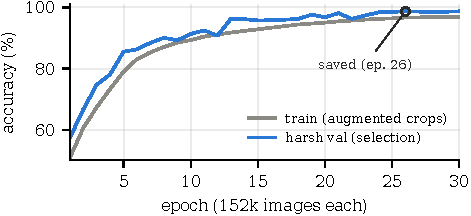
\includegraphics[width=\linewidth]{fig/curves_v4.pdf}
  \caption{\textbf{Training of our model.} Training accuracy on augmented crops and held-out accuracy under the harsh augmentation (used for selection).}
  \label{fig:curves}
\end{figure}

\subsection{Ablations and training behaviour}
\noindent\textbf{Crop size and class rebalancing.} A variant trained with $128^2$ crops and 20 copies of the smoothest 25\% of real images ties our model (dev 96.0\%). Its best-dev checkpoint (97.3\%, epoch 20) predicts 744 test images as real, so on 900 dev images a 1-point gain is noise. We therefore select on harsh validation.

\noindent\textbf{Invariance is slow to learn.} The baseline passes 99.9\% after two epochs of 12k images. Our model needs 21 epochs of 152k crops to pass 98\% on harsh validation (\cref{fig:curves}): invariance must be learnt from many shifted and rescaled examples. The held-out curves track training accuracy, so 30 epochs do not overfit.

\subsection{Error analysis}
\begin{figure}[t]
  \centering
  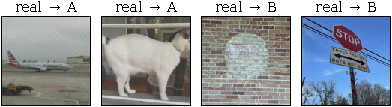
\includegraphics[width=\linewidth]{fig/failures.pdf}
  \caption{\textbf{Most confident errors of our model on dev}: real photographs labelled as Model~A or~B with probability ${>}0.99$. Each scene is ordinary and textured; none shows visible processing.}
  \label{fig:failures}
\end{figure}
The dev confusion matrix of our model (rows: true real/A/B) is
$\left[\begin{smallmatrix}268&10&22\\2&298&0\\1&0&299\end{smallmatrix}\right]$.
32 of its 35 errors are real images called fake. A and B are never confused with each other, and fake recall is 99.5\%. Real recall rises with texture, from 84\% for the smoothest quarter of real images to 92--93\% for the two most textured. Yet the most confident errors (\cref{fig:failures}) are ordinary textured photographs, which suggests our model partly relies on scene statistics of the training reals. On test, our model predicts 36 more real images than exist, so some fakes, plausibly those weakened by re-encoding, are called real. Either way, the errors are real versus fake, not A versus B.
